\documentclass[11pt,]{article}
\usepackage[utf8]{inputenc}
\usepackage{graphicx}
\usepackage{amsmath}
\usepackage{enumitem}
\graphicspath{ {imgs/} }
\usepackage{indentfirst}
\usepackage{float}

\title{Controle Fuzzy}
\author{Jhonantans Moraes Rocha }
\date{Outubro 2016}


\begin{document}

\maketitle

    \section{Fase Mínima}      
    \begin{center}
	     \begin{tabular}{|c|c|}
	            \hline
	            \multicolumn{2}{|c|}{Ponto de operação utilizado} \\
	            \hline\hline
	             A1, A3 & 28 \\ \hline
	             A2, A4 & 32 \\ \hline
	             a1, a3 & 0.071 \\ \hline
	             a2, a4 & 0.057 \\ \hline
	             g & 981 \\ \hline
	             k1 & 3,33 \\ \hline
	             k2 & 3.35 \\ \hline
	             y1 & 0.70 \\ \hline
	             y2 & 0.60 \\ \hline
	            \hline
	        \end{tabular}
	 \end{center}
	
	\subsection{Linearização}    
	    Linearizando em:
	    \begin{figure}[H]
	    	\centering
	    	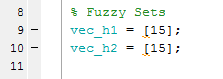
\includegraphics[scale=1]{cod_fuz_15.png}
	    	\caption{Pontos de Linearização}
	    	\label{CodigoLin15}
	    \end{figure}
        
        Sintonizando o controlador LQI na forma:
         \begin{figure}[H]
         	\centering
         	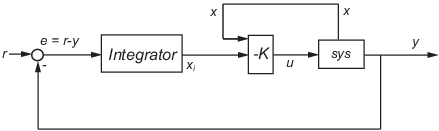
\includegraphics[scale=1]{lqi1.png}
         	\caption{Esquemático do Sistema em Malha Fechada}
         	\label{EsqLQI}
         \end{figure}
        Onde utiliza-se como entrada do canal integrador o erro entre as referências e os níveis $h_1$ e $h_2$.
        Para a sintonia do controlador, são necessárias as matrizes Q e R, onde:
        \begin{align*}
        	Q &= 
        	\begin{bmatrix}
        		1 & 0 & 0 & 0 \\
        		0 & 1 & 0 & 0 \\
        		0 & 0 & 1 & 0 \\
        		0 & 0 & 0 & 1
        	\end{bmatrix} \\
			R &= 
        	\begin{bmatrix}
	        	1 & 0 \\
	        	0 & 1
        	\end{bmatrix}
        \end{align*}
        
        Temos:
        \begin{align*}
	        -K &= 
	        \begin{bmatrix}
	        -4.8384 & 0.0849 & -0.4874 & 0.0004 & 0.9999 & -0.0118\\
		    -0.0413 & -5.6072 & -0.0125 & -0.4663 & 0.0118 & 0.9999
	        \end{bmatrix}
        \end{align*}
        
        Simulando o controlador desenvolvido sobre o sistema não-linear, obtem-se:
         \begin{figure}[H]
               	\centering
               	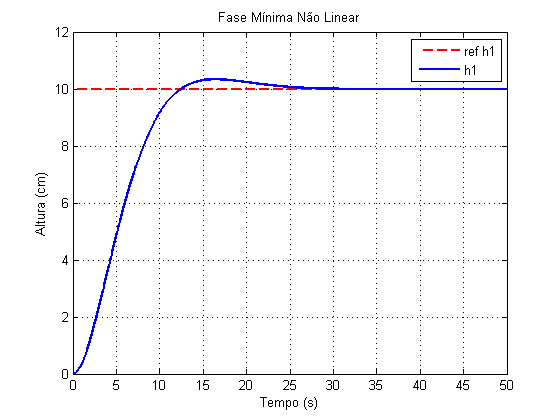
\includegraphics[scale=1]{h1_lin15.png}
               	\caption{Resposta do nível h1 para a referência}
               	\label{H1_lin15}
         \end{figure}
         \begin{figure}[H]
         	\centering
         	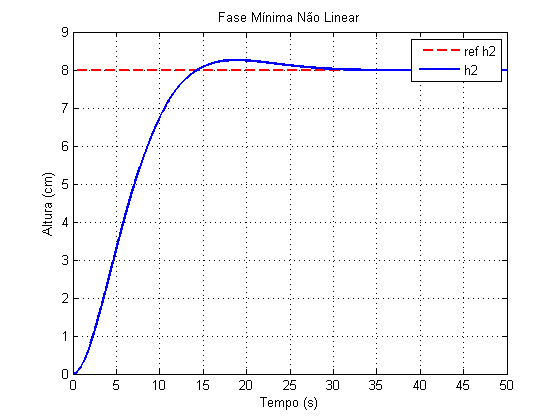
\includegraphics[scale=1]{h2_lin15.png}
         	\caption{Resposta do nível h2 para a referência}
         	\label{H2_lin15}
         \end{figure}

	\subsection{Modelagem Fuzzy}    
    Seguindo o mesmo princípio, desenvolve-se controladores para cada uma das combinações dos modelos a seguir:
	\begin{figure}[H]
		\centering
		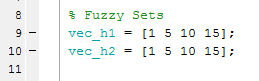
\includegraphics[scale=1]{cod_fuz_1_5_10_15.png}
		\caption{Pontos de Linearização Fuzzy}
		\label{CodigoLinFuzzy}
	\end{figure}
	
	Obtém-se um total de 4x4 = 16 matrizes K. Aplicando-se o controle fuzzy sobre o sistema não-linear, obtém-se:
	\begin{figure}[H]
		\centering
		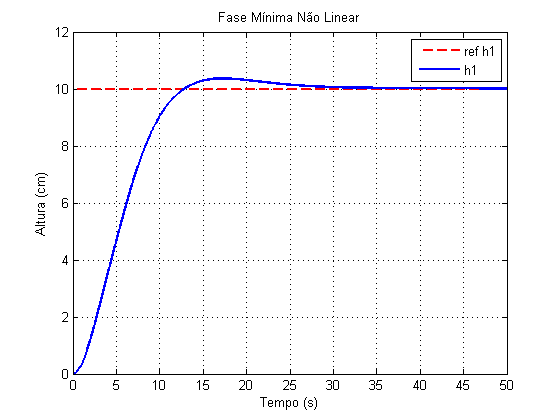
\includegraphics[scale=1]{h1_fuz_fm.png}
		\caption{Resposta do nível h1 para a referência}
		\label{h1_fuz_fm}
	\end{figure}
	\begin{figure}[H]
		\centering
		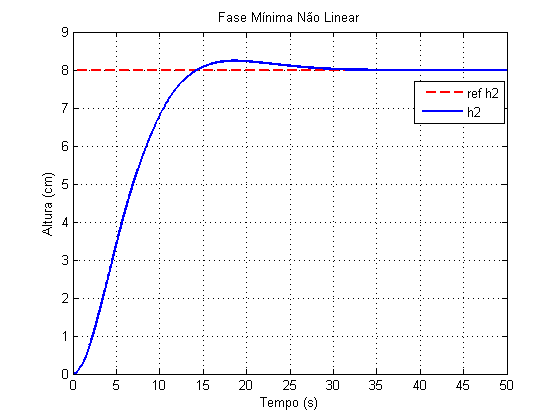
\includegraphics[scale=1]{h2_fuz_fm.png}
		\caption{Resposta do nível h2 para a referência}
		\label{h2_fuz_fm}
	\end{figure}
	
	\subsection{Comparação}
	Comparando os resultados para o níveil $h_1$ em uma única imagem, nota-se uma leve diferença:
	\begin{figure}[H]
		\centering
		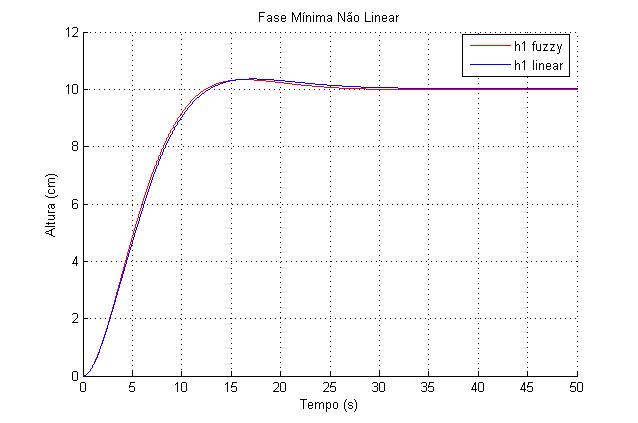
\includegraphics[scale=1]{h1_comp.png}
		\caption{Comparação para h1}
		\label{h1_comp}
	\end{figure}
	\begin{figure}[H]
		\centering
		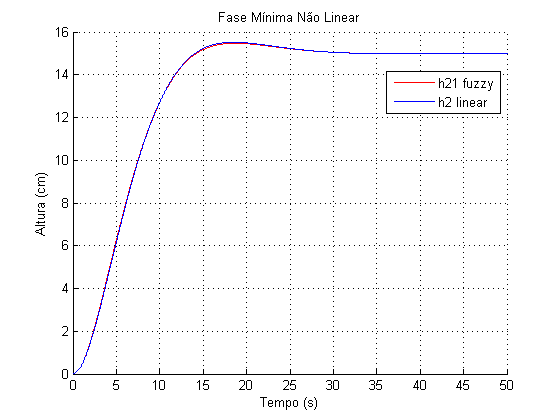
\includegraphics[scale=1]{h2_comp.png}
		\caption{Comparação para h2}
		\label{h2_comp}
	\end{figure}

	Como pode ver, o ganho pela utilização fuzzy foi muito pequeno, uma vez que os K obtidos para cada um dos sistemas foi praticamente idêntico.
	
	\section{Fase Não Mínima}      
	\begin{center}
		\begin{tabular}{|c|c|}
			\hline
			\multicolumn{2}{|c|}{Ponto de operação utilizado} \\
			\hline\hline
			A1, A3 & 28 \\ \hline
			A2, A4 & 32 \\ \hline
			a1, a3 & 0.071 \\ \hline
			a2, a4 & 0.057 \\ \hline
			g & 981 \\ \hline
			k1 & 3,15 \\ \hline
			k2 & 3.29 \\ \hline
			y1 & 0.43 \\ \hline
			y2 & 0.34 \\ \hline
			\hline
		\end{tabular}
	\end{center}
	
	\subsection{Linearização}    
	Linearizando em:
	\begin{figure}[H]
		\centering
		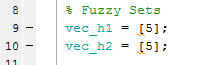
\includegraphics[scale=1]{cod_fuz_05.png}
		\caption{Pontos de Linearização}
		\label{CodigoLin05_2}
	\end{figure}

	E sintonizando o controlador da mesma forma que anterior, obtemos:
	\begin{align*}
	-K &= 
	\begin{bmatrix}
	14.9984 & -30.1819 & 13.2258 & -18.4241 & 0.1469 & 0.9892\\
	-23.8928 & 27.2788 & -15.8981 & 20.0756 & 0.9892 & -0.146
	\end{bmatrix}
	\end{align*}
	
	Simulando o controlador desenvolvido sobre o sistema não-linear, obtem-se:
	\begin{figure}[H]
		\centering
		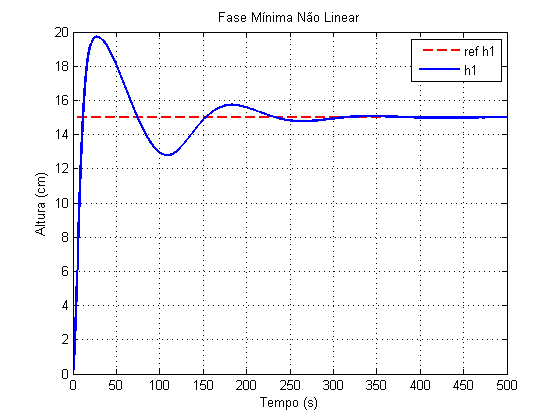
\includegraphics[scale=1]{h1_lin05_nm.png}
		\caption{Resposta do nível h1 para a referência}
		\label{H1_lin05_nm}
	\end{figure}
	\begin{figure}[H]
		\centering
		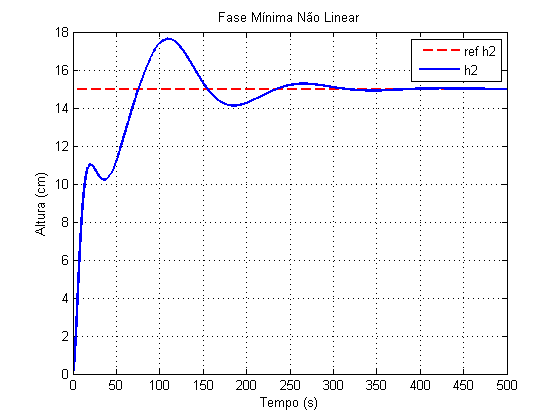
\includegraphics[scale=1]{h2_lin05_nm.png}
		\caption{Resposta do nível h2 para a referência}
		\label{H2_lin05_nm}
	\end{figure}
	
	Para outro ponto, em:
	\begin{figure}[H]
		\centering
		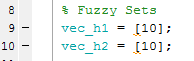
\includegraphics[scale=1]{cod_fuz_10.png}
		\caption{Pontos de Linearização}
		\label{CodigoLin10}
	\end{figure}
	
	E sintonizando o controlador da mesma forma que anterior, obtemos:
	\begin{align*}
	-K &= 
	\begin{bmatrix}
	22.1950 & -40.9672 & 18.1821 & -24.6981 & 0.1593 & 0.9872\\
	-32.8634 & 40.1285 & -21.6964 & 27.9406  & 0.9872 & -0.1593
	\end{bmatrix}
	\end{align*}
	
	Simulando o controlador desenvolvido sobre o sistema não-linear, obtem-se:
	\begin{figure}[H]
		\centering
		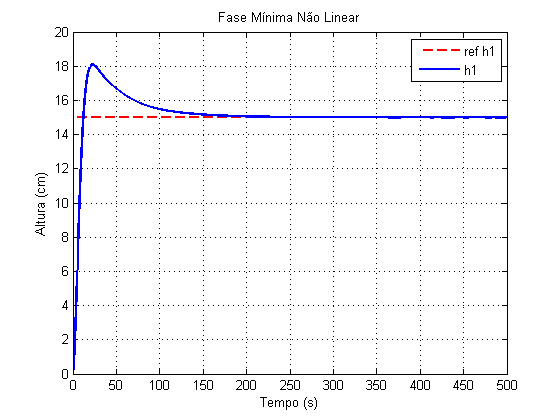
\includegraphics[scale=1]{h1_lin10_nm.png}
		\caption{Resposta do nível h1 para a referência}
		\label{H1_lin10_nm}
	\end{figure}
	\begin{figure}[H]
		\centering
		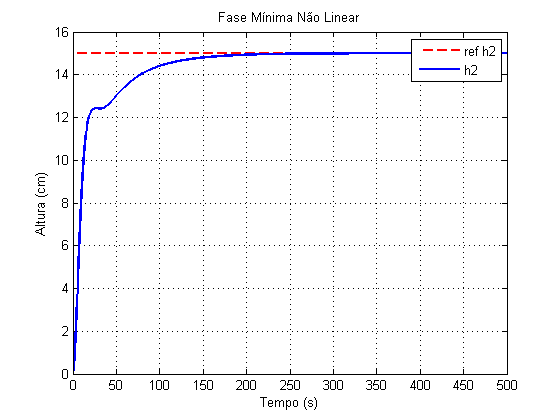
\includegraphics[scale=1]{h2_lin10_nm.png}
		\caption{Resposta do nível h2 para a referência}
		\label{H2_lin10_nm}
	\end{figure}
	
	Para um terceiro ponto, em:
	\begin{figure}[H]
		\centering
		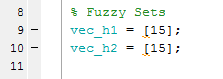
\includegraphics[scale=1]{cod_fuz_15.png}
		\caption{Pontos de Linearização}
		\label{CodigoLin15_2}
	\end{figure}
	
	E sintonizando o controlador da mesma forma que anterior, obtemos:
	\begin{align*}
	-K &= 
	\begin{bmatrix}
	 27.7556 & -49.1931 & 21.9359 & -29.5209 & 0.1651 & 0.9863\\
	 -39.7251 & 50.0135 & -26.1520 & 33.9199 & 0.9863 & -0.1651
	\end{bmatrix}
	\end{align*}
	
	Simulando o controlador desenvolvido sobre o sistema não-linear, obtem-se:
	\begin{figure}[H]
		\centering
		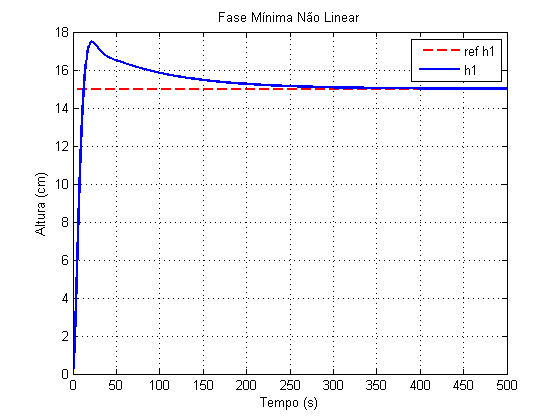
\includegraphics[scale=1]{h1_lin15_nm.png}
		\caption{Resposta do nível h1 para a referência}
		\label{H1_lin15_nm}
	\end{figure}
	\begin{figure}[H]
		\centering
		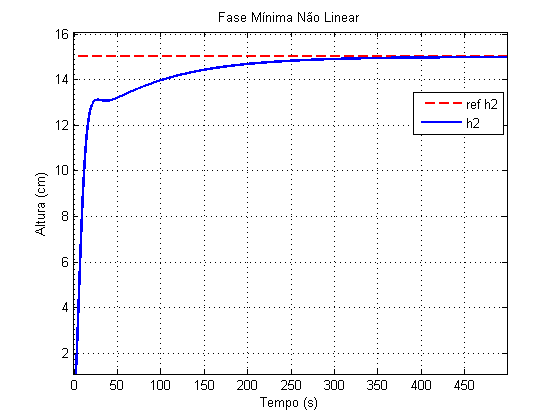
\includegraphics[scale=1]{h2_lin15_nm.png}
		\caption{Resposta do nível h2 para a referência}
		\label{H2_lin15_nm}
	\end{figure}
	
	\subsection{Modelagem Fuzzy}    
	Seguindo o mesmo princípio, desenvolve-se controladores para cada uma das combinações dos modelos a seguir:
	\begin{figure}[H]
		\centering
		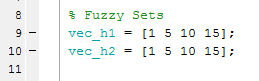
\includegraphics[scale=1]{cod_fuz_1_5_10_15.png}
		\caption{Pontos de Linearização Fuzzy}
		\label{CodigoLinFuzzy_2}
	\end{figure}
	
	Obtém-se um total de 4x4 = 16 matrizes K. Aplicando-se o controle fuzzy sobre o sistema não-linear, obtém-se:
	\begin{figure}[H]
		\centering
		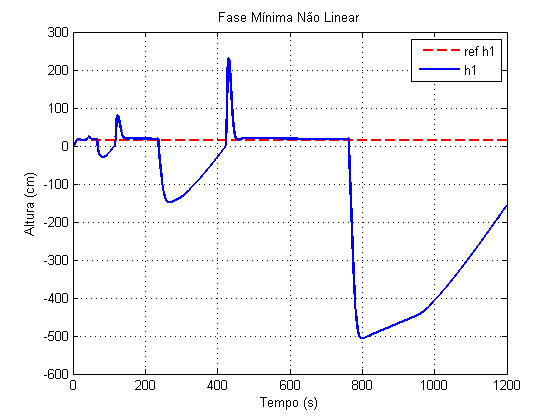
\includegraphics[scale=1]{h1_fuz_nm.png}
		\caption{Resposta do nível h1 para a referência}
		\label{h1_fuz_nm}
	\end{figure}
	\begin{figure}[H]
		\centering
		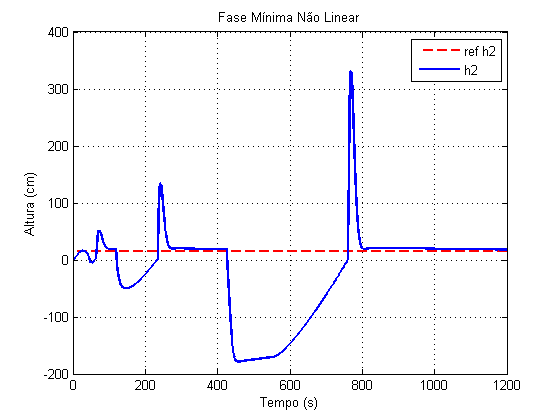
\includegraphics[scale=1]{h2_fuz_nm.png}
		\caption{Resposta do nível h2 para a referência}
		\label{h2_fuz_nm}
	\end{figure}
	
	\subsection{Modelagem Fuzzy}    
	Estou procurando o motivo para tamanha discrepância do sistema fuzzy. Pode haver algum erro no meu código, estou o apurando. Mesmo assim se houvesse, deveria aparecer também o sistema em fase mínima, o que não é caso.
	Se não for este o motivo, qual poderia ser? Os K para o não linear variam muito de um sistema para o outro, o que torna suas respostas muito diferentes, mesmo assim, com um controlador simples o sistema final de todos se estabiliza, enquanto o fuzzy não.
	Vou verificar como o sistema se comporta para cada um dos 16 ganhos individualmente. Também preciso apurar as matrizes Q e R que utilizo para o desenvolvimento dos controladores.

                            
\end{document}
